\chapter{設計と実装}
本性では,提案ツールを開発するときのアプローチを述べる.

\section{提案ツールの設計}

\section{開発環境}
提案ツールの開発環境を下記に示す.

\begin{itemize}
    \item OS:macOS Big Sur 11.1
    \item プログラミング言語:Python 3.7
    \item 統合開発環境:PyCharm 2020.3.2
\end{itemize}

\section{実装規模}

\section{提案ツールのアーキテクチャ}
\begin{figure}[H]
    \centering
    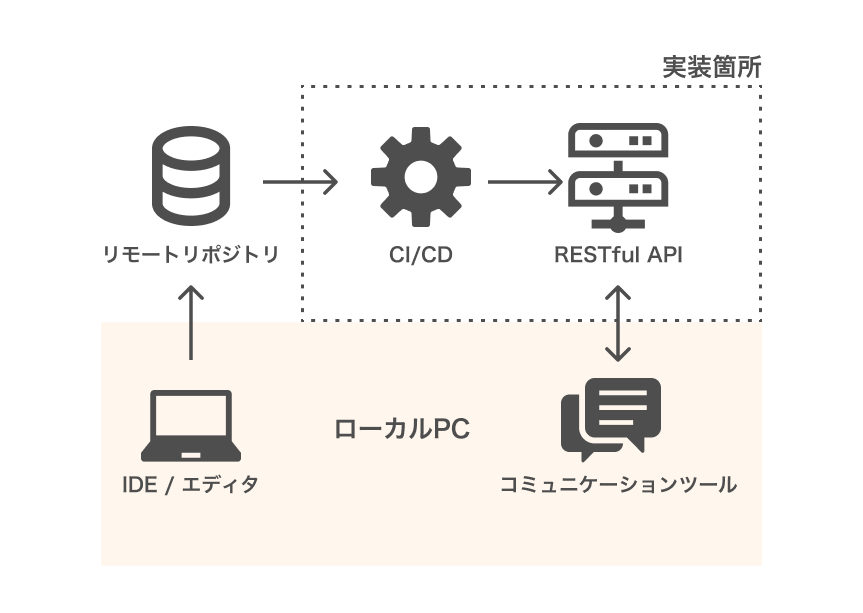
\includegraphics[width=12cm]{images/architecture.png}
    \caption{提案ツールのアーキテクチャ}
    \label{architecture}
\end{figure}

提案ツールのアーキテクチャを図\ref{architecture}に示す.
提案ツールのmilkは,既存のCI/CDツール上で動作することを想定しており,CI/CDツールにはGitHub Actionsを用いた.
CI/CDツール上でできることが限られているため,同時に,Slackとのやりとりや,開発プロジェクトの状態の管理を行うことができるRESTful APIの開発も行った.
RESTful APIにはFastAPIを使用し,各種データの保持はJSONファイルのI/Oにて管理を行っている.
また,RESTful APIは筆者のローカルPC上で動作させているが,HTTPSとして外部公開させることができるツールのngrokを使用しており,
Slack APIやCI/CD上で動作するmilkはローカルPC上で動作するRESTful APIを使用できるようになっている.

RESTful APIには,下記の機能をもたせているが,乖離検知の処理はすべてmilkで行う

\begin{itemize}
    \item 各機能のステータスを更新する機能
    \item Gitのコミットの差分量を追加する機能
    \item SlackのAPIを呼び出してメッセージを送受信する機能
\end{itemize}

開発者は,適切なタイミングで変更を記録するためにコミットを実行し,リモートリポジトリにプッシュすることを期待している.
リモートリポジトリにプッシュされたタイミングで,CI/CDツールが起動し,CI/CDツールの設定ファイルに定義されたコマンドが実行される.
このとき,Pythonで作成したmilkコマンドを実行するために,CI/CDツール上でPython環境を構築している.
乖離リスクの検知を行うために,まずRESTful APIから開発プロジェクトの現状態を取得する.
その後,C1~C4について乖離リスクの検知を行い,検知したときにRESTful APIを通じてSlackへとメッセージを送信する.




Slackにmilkコマンドが入力されると,SlackからRESTful APIにHTTPリクエストを行われるため,これを適切にハンドリングすることでJSONファイルに値を書き込むことができる.

\section{提案ツールの使用方法}

\section{コミュニケーションツールで利用可能なコマンド}
milkでは,Slackのスラッシュコマンドを活用することで,各種パラメータの設定を行うことができるようになっている.
以下では,milkで使用可能なコマンドをまとめる.

\subsection*{/milk c1 doc [ file type ]}
ソースコード先行検知の機能において,開発プロジェクトで使用するSwaggerドキュメントのファイル形式を指定することができるコマンドである.
本コマンドは,開発プロジェクトの初期段階でSwaggerドキュメントのファイル形式を指定する場合や,開発プロジェクトの途中でファイル形式を変更したい場合に利用されることを想定している.

\subsection*{/milk c1 code [ file type ]}
ソースコード先行検知の機能において,開発プロジェクトで使用するプログラミング言語を指定することができるコマンドである.
現在では,プログラミング言語にPythonのみを指定可能である.

\subsection*{/milk c1 param}
ソースコード先行検知の機能において,現在設定しているSwaggerドキュメントの拡張子および使用しているプログラミング言語の拡張子を確認することができるコマンドである.

\subsection*{/milk c2 set [ days ]}
一定時間経過後のリマインダーの機能において,ドキュメントが更新されずソースコードのみが更新されている場合に,ドキュメントを追加・修正するためのリマインダーを行う間隔を指定することができるコマンドである.

\subsection*{/milk c2 param}
一定時間経過後のリマインダーの機能において,現在設定しているリマインダーを行う間隔を確認することができるコマンドである.

\subsection*{/milk c3 set [ version file ]}
リリース時ドキュメント更新有無の検知の機能において,バージョンを扱うファイルを指定することができるコマンドである.
例えば,Pythonではsetup.pyと呼ばれるファイルにソフトウェアのバージョンを記述している.
現在では,バージョンを扱うファイルにsetup.pyのみを指定可能である.

\subsection*{/milk c4 set [ number ]}
ソースコード変更量の検知の機能において,ドキュメントが更新されずソースコードのみが更新されている場合に,ソースコードの追加・削除・修正が行われた行数を指定することができるコマンドである.
指定した行数を超過してソースコードのみを記述し続けたときに通知がでる.

\subsection*{/milk c4 param}
ソースコード変更量の検知の機能において,現在設定している変更量を確認することができるコマンドである.
